\documentclass[../AP_Calculus]{subfiles}

\begin{document}
	\section{Parametric Equations}
		A \textbf{parametric equation} defines its independent and dependent variables in terms of the same parameter, often $t$.
		\callout{17}{A parametric graph should have arrows going through it showing the direction of $t$. It should not have arrows showing end behavior.}
		To graph a parametric function, $t$ can be swept or the parameter can be eliminated by solving for it in terms of one of the variables.
		\subsection{Parametric Derivatives}
		The derivative of a parametric equation is still taken, unless otherwise specified, with respect to time.
		\[\frac{\d y}{\d x} = \frac{\frac{\d y}{\d t}}{\frac{\d x}{d t}}\]
		The second derivative of a parametric equation is the time is the first derivative differentiated with respect to $t$ divided by $\d x/\d t$.
		\[\frac{\d^2y}{\d x^2} = \frac{\frac{\d}{\d t}\frac{\d y}{\d x}}{\frac{\d x}{\d t}}\]
		The $\nth{n}$ derivative of a parametric equation takes the following form: \\
		\subsection{Parametric Arc Length}
			\textbf{Rectangular arc length} is defined as such:
			\[L = \int_a^b\sqrt{1 + \left(\frac{\d y}{\d x}\right)^2}\d x\]
		\textbf{Parametric arc length} is differentiated with respect to $t$:
		\[L = \int_a^b\sqrt{\left(\frac{\d x}{\d t}\right)^2 + \left(\frac{\d y}{\d t}\right)^2}\d t\]
	\section{Polar Equations}
		A \textbf{polar} function is written using 
		\textbf{Circular coordinates} denote values as an ordered pair of its distance from the origin (the \textbf{radial line} and its angle relative to what would be the positive $x$-axis in the cartesian plane.
		\begin{center}
			\begin{tikzpicture}
				\draw[<->] (-4, 0) -- (4, 0);
				\draw[<->] (0, -4) -- (0, 4);
				\fill (3, 3) circle (2pt);
				\node[right] at (3, 3.25) {$(r, \theta)$};
				\draw[dashed] (0, 0) -- (3, 3);
				\coordinate (a) at (3, 3);
				\coordinate (b) at (0, 0);
				\coordinate (c) at (4, 0);
				\draw pic[draw, ->, angle radius = 1cm, "$\theta$"]{angle = c--b--a};
				\draw[|-|] (-0.4, 0.1) -- node[left]{$r$} (2.8, 3.3);
			\end{tikzpicture}
		\end{center}
		Polar coordinates can be written in infinite ways by adding or subtracting integer multiples of $2\pi$. \\
		\[(r, \theta) \equiv (r, \theta \pm 2z\pi) \forall z \in \mathbb{Z}\]
		To convert from polar to cartesian coordinates, trigonometric functions can be used.
		\[\overset{\text{polar}}{(r, \theta)} \implies \overset{\text{cartesian}}{(r\cos\theta, r\sin\theta)}\]
		Inverse tangent and the Pythagorean theorem can be used perform the converse process.
		\[\overset{\text{cartesian}}{(x, y)} \implies \overset{\text{polar}}{\left(\sqrt{x^2 + y^2}, \arctan\left(\frac{y}{x}\right)\right)}\]
		Radii can be negative, reflecting it over the origin. A negative radius is equivalent to an additional rotation of $\pi$.
		\begin{center}
			\begin{tikzpicture}
				\draw[<->] (-4, 0) -- (4, 0);
				\draw[<->] (0, -4) -- (0, 4);
				\fill (3, 3) circle (2pt);
				\node[right] at (3, 3.25) {$(-r, \theta)$};
				\node[left] at (-3, -3.25) {$(r, \theta)$};
				\draw[dashed] (-3, -3) -- (3, 3);
				\coordinate (a) at (-3, -3);
				\coordinate (b) at (0, 0);
				\coordinate (c) at (4, 0);
				\coordinate (d) at (3, 3);
				\draw pic[draw, ->, angle radius = 0.6cm, "$\theta$"]{angle = c--b--a};
				\draw pic[draw, ->, angle radius = 1cm, "$+\pi$"]{angle = a--b--d};
				\draw pic[draw, <-, angle radius = 1.4cm, "$-\pi$" shift = {(-1mm, 1mm)}]{angle = d--b--a};
			\end{tikzpicture}
		\end{center}
		\subsection{General Forms}
			Polar equations come in four general forms:
			\begin{itemize}
				\item There are three types of \textbf{circles}:
					\begin{itemize}
						\item $r = a$ is a circle centered about the origin with radius $|a|$.
							\begin{center}
								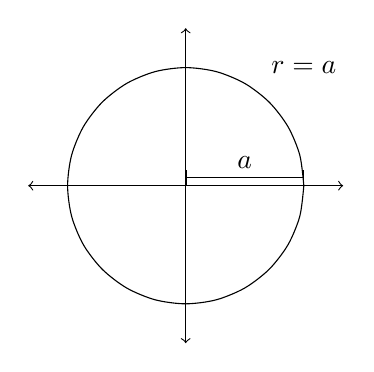
\begin{tikzpicture}
									\draw[<->] (-2, 0) -- (2, 0);
									\draw[<->] (0, -2) -- (0, 2);
									\draw[domain = 0:{2 * pi}, smooth] plot({deg(\x)}:{1.5});
									\node at (1.5, 1.5){$r = a$};
									\draw[|-|] (0, 0.1) -- node[above]{$a$} ++ (1.5, 0);
								\end{tikzpicture}
							\end{center}
						\item $r = a\cos\theta$ is a circle tangent to the origin on the horizontal axis with radius $\frac{|a|}{2}$.
							\begin{center}
								\begin{tikzpicture}
									\draw[<->] (-2, 0) -- (2, 0);
									\draw[<->] (0, -2) -- (0, 2);
									\draw[domain = 0:pi, smooth] plot({deg(\x)}: {1.5 * cos(deg(\x))});
									\draw[|-|] (0, 0.1) -- node[above]{$|a|$} ++ (1.5, 0);
									\node at (1.1, 1.3) {$r = a\cos\theta$};
								\end{tikzpicture}
							\end{center}
						\item $r = a\sin\theta$ is a circle tangent to the origin on the vertical axis with radius $\frac{|a|}{2}$.
							\begin{center}
								\begin{tikzpicture}
									\draw[<->] (-2, 0) -- (2, 0);
									\draw[<->] (0, -2) -- (0, 2);
									\draw[domain = 0:pi, smooth] plot({deg(\x)}:{1.5 * sin(deg(\x))});
									\draw[|-|] (0.1, 0) -- node[right]{$|a|$} ++ (0, 1.5);
								\end{tikzpicture}
							\end{center}
					\end{itemize}
				\item \textbf{Limacons} take the form of $r = a\pm b\sin\theta$ or $r = a\pm b\cos\theta$ ($a, b > 0$), which are symmetrical about the vertical or horizontal axis respectively. There are four cases for them:
					\begin{itemize}
						\item If $\frac{a}{b} < 1$, there is a loop passing through the origin and $(a + b, 0)$ in addition to another loop passing through the origin and $(b - a, 0)$.
							\begin{center}
								\begin{tikzpicture}
									\draw[<->] (-2, 0) -- (2, 0);
									\draw[<->] (0, -2) -- (0, 2);
								\end{tikzpicture}
							\end{center}
						\item If $\frac{a}{b} = 1$, the graph is a \textbf{cardioid}, passing through the origin, $\left(\pm a, \frac{\pi}{2}\right)$, and $(2a, 0)$.
							\begin{center}
								\begin{tikzpicture}
									\draw[<->] (-2, 0) -- (2, 0);
									\draw[<->] (0, -2) -- (0, 2);
								\end{tikzpicture}
							\end{center}
						\item If $1 < \frac{a}{b} < 2$, the graph is \textbf{dimpled}, passing through $(a + b, 0)$, $\left(\pm a, \frac{\pi}{2}\right)$.
							\begin{center}
								\begin{tikzpicture}
									\draw[<->] (-2, 0) -- (2, 0);
									\draw[<->] (0, -2) -- (0, 2);
								\end{tikzpicture}
							\end{center}
						\item If $\frac{a}{b} > 2$, the graph is \textbf{convex}.
							\begin{center}
								\begin{tikzpicture}
									\draw[<->] (-2, 0) -- (2, 0);
									\draw[<->] (0, -2) -- (0, 2);
								\end{tikzpicture}
							\end{center}
					\end{itemize}
				\item \textbf{Rose curves} take the form of $r = a\sin(n\theta)$ or $r = a\cos(n\theta)$, which are symmetrical about the vertical or horizontal axis respectively. The location of a petal can be found by equation the trigonometric term to 1 while the distance between from the origin to the tip of any given petal is $a$. There are two cases for rose curves:
					\begin{itemize}
						\item If $n$ is odd, there are $n$ evenly spaced petals.
							\begin{center}
								\begin{tikzpicture}
									\draw[<->] (-2, 0) -- (2, 0);
									\draw[<->] (0, -2) -- (0, 2);
								\end{tikzpicture}
							\end{center}
						\item If $n$ is even and at least 2, there are $2n$ evenly spaced petals.
							\begin{center}
								\begin{tikzpicture}
									\draw[<->] (-2, 0) -- (2, 0);
									\draw[<->] (0, -2) -- (0, 2);
								\end{tikzpicture}
							\end{center}
					\end{itemize}
				\item \textbf{Lemniscates} take the form of $r^2 = a^2\sin(n\theta)$ or $r^2 = a^2\cos(n\theta)$, are symmetrical about $\theta = \frac{\pi}{4}$ or the horizontal axis respectively.
					\begin{itemize}
						\item If $n$ is odd, there are $2n$ petals.
							\begin{center}
								\begin{tikzpicture}
									\draw[<->] (-2, 0) -- (2, 0);
									\draw[<->] (0, -2) -- (0, 2);
								\end{tikzpicture}
							\end{center}
						\item If $n$ is even, there are $n$ petals.
							\begin{center}
								\begin{tikzpicture}
									\draw[<->] (-2, 0) -- (2, 0);
									\draw[<->] (0, -2) -- (0, 2);
								\end{tikzpicture}
							\end{center}
					\end{itemize}
			\end{itemize}
\end{document}